%----------------------------------------------------------------------------------------
%	PACKAGES AND DOCUMENT CONFIGURATIONS
%----------------------------------------------------------------------------------------

\documentclass{article}

%\usepackage[version=3]{mhchem} % Package for chemical equation typesetting
\usepackage{siunitx} % Provides the \SI{}{} and \si{} command for typesetting SI units
\usepackage{graphicx} % Required for the inclusion of images
%\usepackage{natbib} % Required to change bibliography style to APA
\usepackage{amsmath} % Required for some math elements 

\setlength\parindent{0pt} % Removes all indentation from paragraphs
\usepackage{float}
\usepackage[a4paper, total={7in, 8in}]{geometry}
%\renewcommand{\labelenumi}{\alph{enumi}.} % Make numbering in the enumerate environment by letter rather than number (e.g. section 6)

%\usepackage{times} % Uncomment to use the Times New Roman font

% For letter numbering
\renewcommand{\thesubsubsection}{\alph{subsubsection})}
\makeatletter
\renewcommand{\p@subsubsection}{\thesubsection.\protect\eatbracket}
\makeatother
\def\eatbracket#1#2{#1\ifx)#2\else#2\fi}

% Math symbols
\usepackage{amsfonts}

% Graphics path
\graphicspath{{Section1/}{Section2/}}
%----------------------------------------------------------------------------------------
%	DOCUMENT INFORMATION
%----------------------------------------------------------------------------------------

\title{4G3 Computational Neuroscience Assignment 1 } % Title

\author{Candidate No: \textsc{5660E}} % Author name

\date{\today} % Date for the report

\begin{document}
	
	\maketitle % Insert the title, author and date
	

	
	%----------------------------------------------------------------------------------------
	%	SECTION 1
	%----------------------------------------------------------------------------------------
	
%	\section{Introduction}
%	The aim of this coursework is to design controllers to stabilize a plant and meet design specifications for its response. (see coursework handout for further details)
	
\section{Network Dynamics}
	
\subsection{Input amplification and integration with a feed-forward linear network}


%	\begin{equation*}
%	K_b = \sqrt{10} \frac{(s + \frac{1}{\sqrt{10}})}{s + \sqrt{10}}\end{equation*}
	
	\subsubsection{Firing rates with $\lambda = 1$}
	
		\begin{figure}[H] 
			\begin{center}
				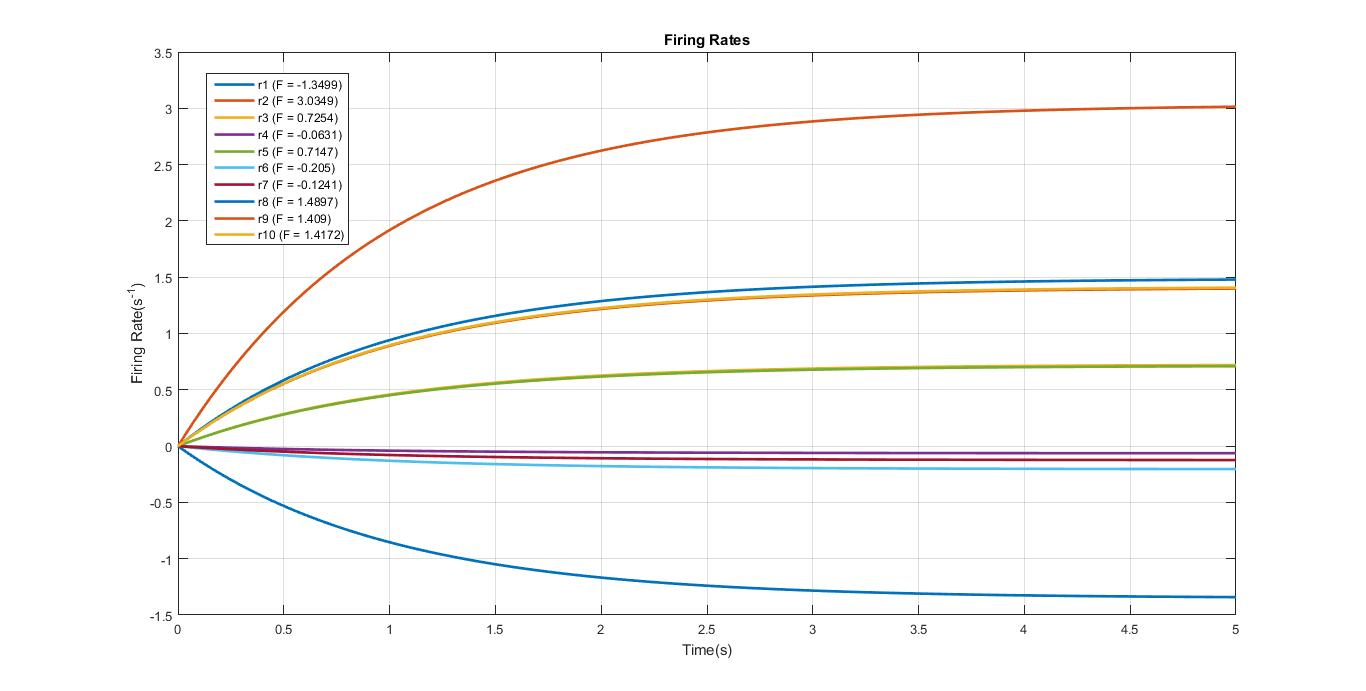
\includegraphics[width=0.9\textwidth]{Section1/Part1/Q1a.jpg}
				\caption{Caption \label{Q1a}}
								\end{center}
		\end{figure}
	
	\subsubsection{Firing rates with $\lambda = 0$}

	\begin{figure}[H] 
		\begin{center}
			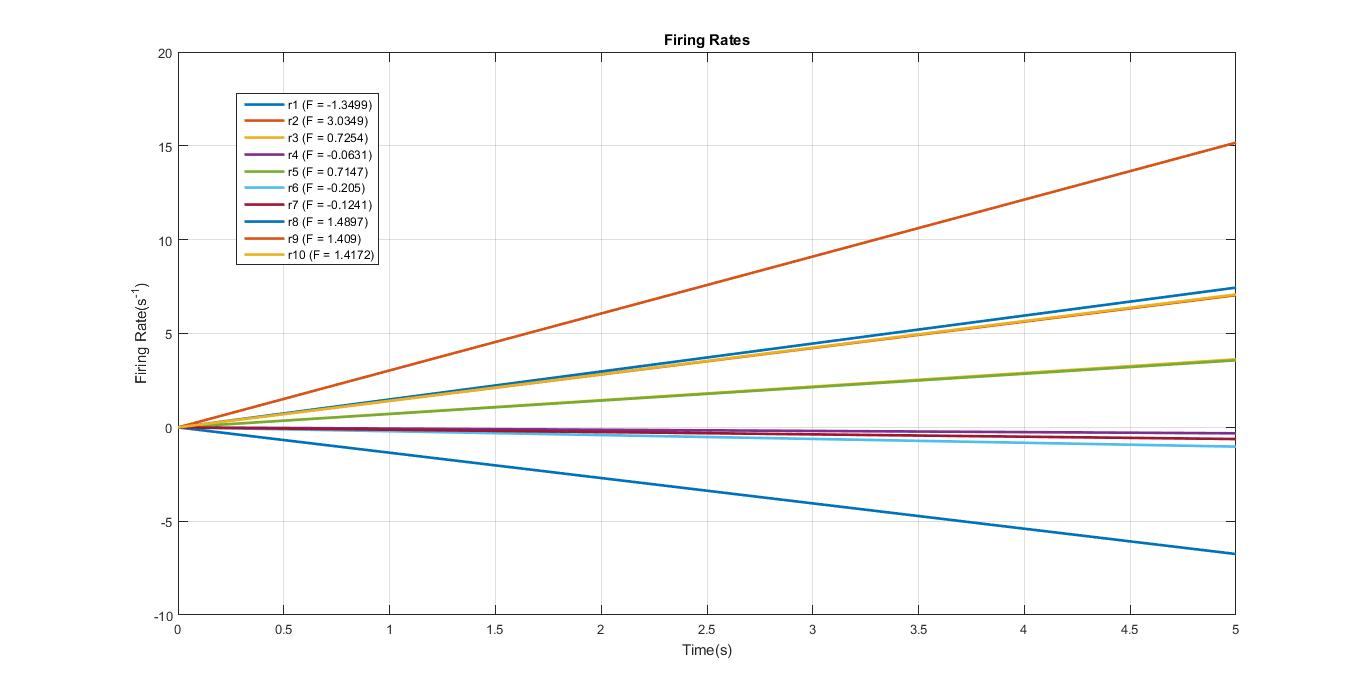
\includegraphics[width=0.9\textwidth]{Section1/Part1/Q1b.jpg}
			\caption{Caption \label{Q1b}}
		\end{center}
	\end{figure}
	
	\subsubsection{Firing rates with $\lambda = -1$}
	
	\begin{figure}[H] 
		\begin{center}
			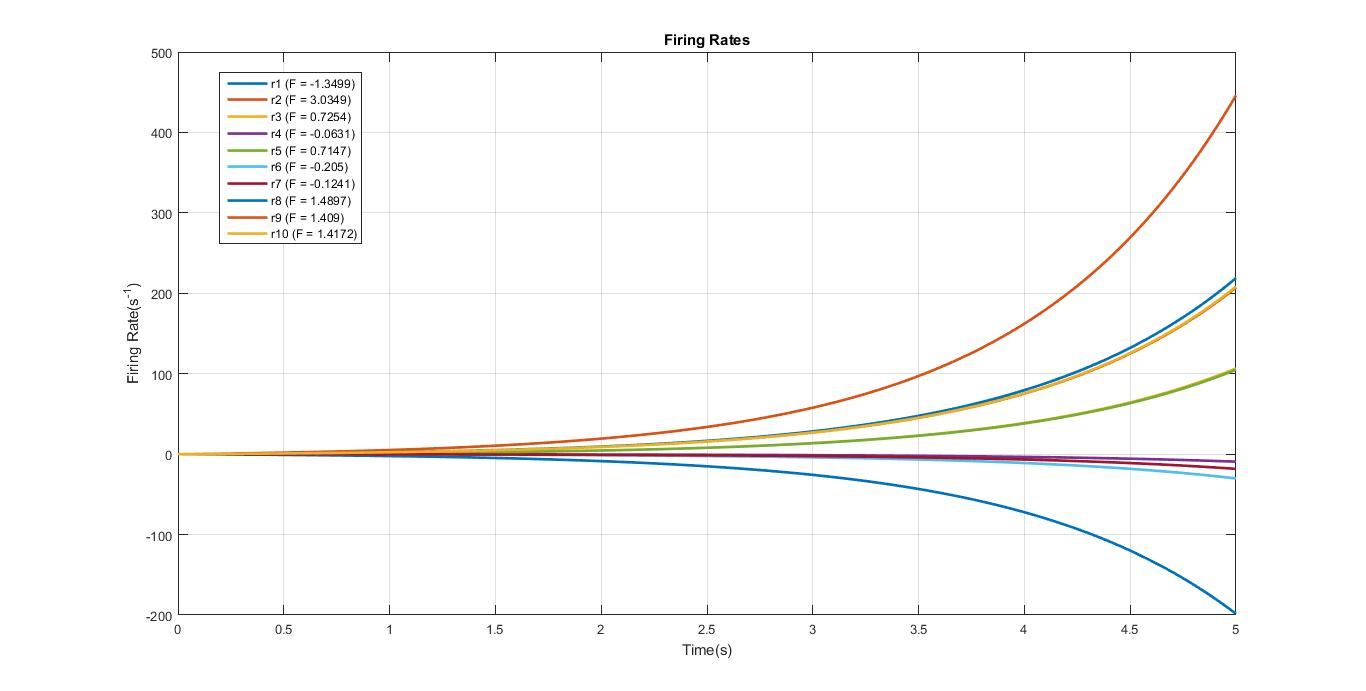
\includegraphics[width=0.9\textwidth]{Section1/Part1/Q1c.jpg}
			\caption{Caption \label{Q1c}}
		\end{center}
	\end{figure}
	
	\subsubsection{Equilibrium firing rates with $\lambda = 1$}
	
	\begin{figure}[H] 
		\begin{center}
			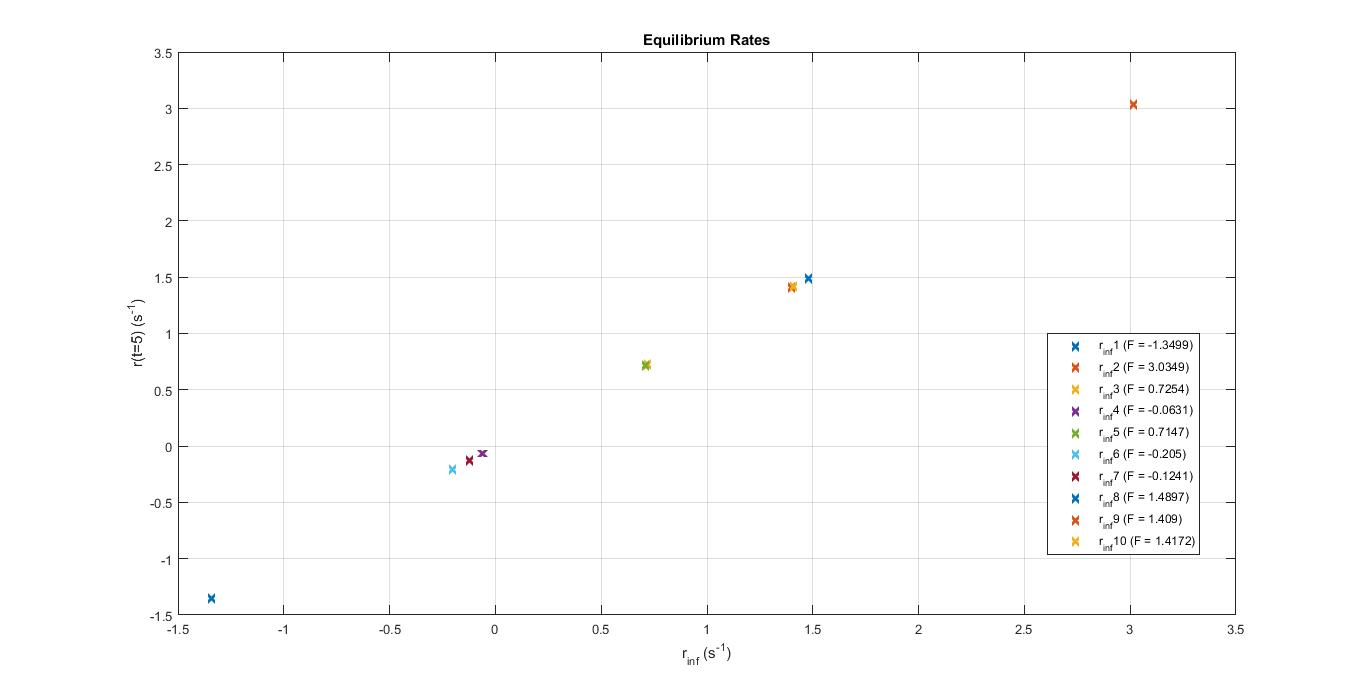
\includegraphics[width=0.9\textwidth]{Section1/Part1/Q1d.jpg}
			\caption{Caption \label{Q1d}}
		\end{center}
	\end{figure}
	
\subsection{Randomly connected network}

\subsubsection{Firing rates with $g = 0$}
i. 
\begin{figure}[H] 
\begin{center}
	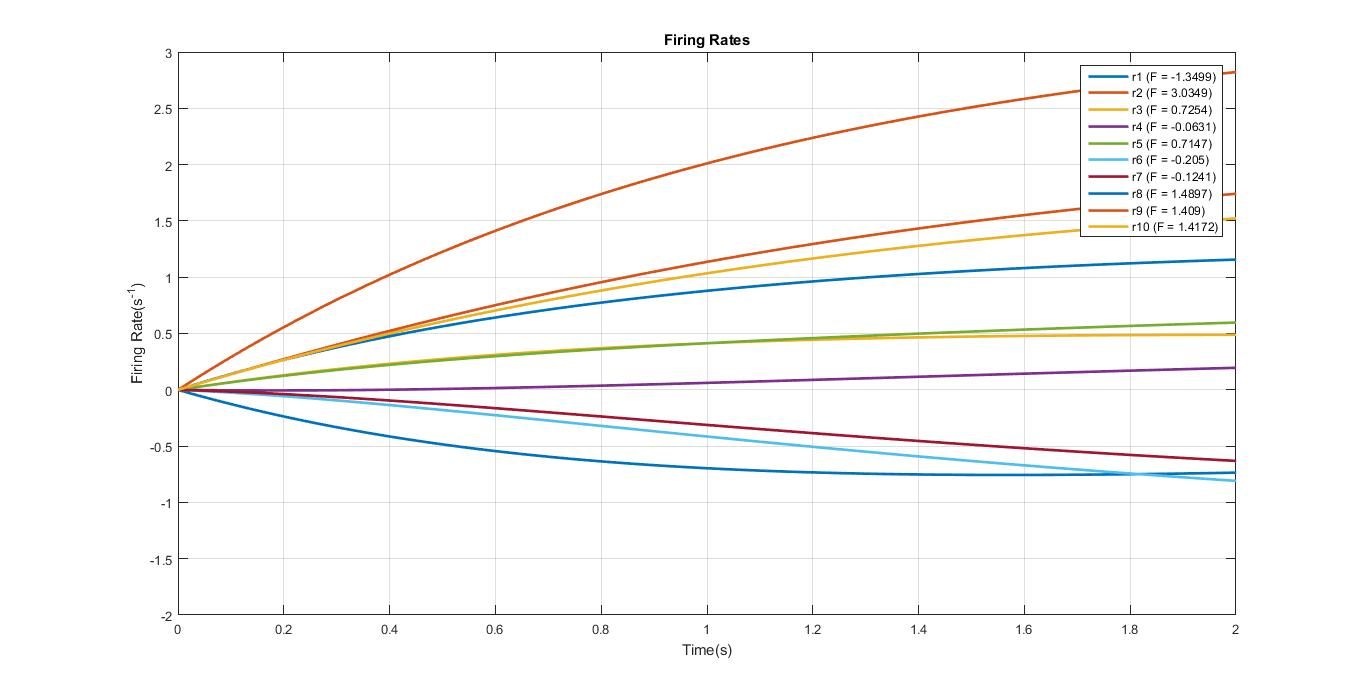
\includegraphics[width=0.9\textwidth]{Section1/Part2/Retry/Q2a_i.jpg}
	\caption{Caption \label{Q2a_i}}
\end{center}
\end{figure}

ii. Eigenvalues of the recurrent connectivity matrix $W$
\begin{figure}[H] 
	\begin{center}
		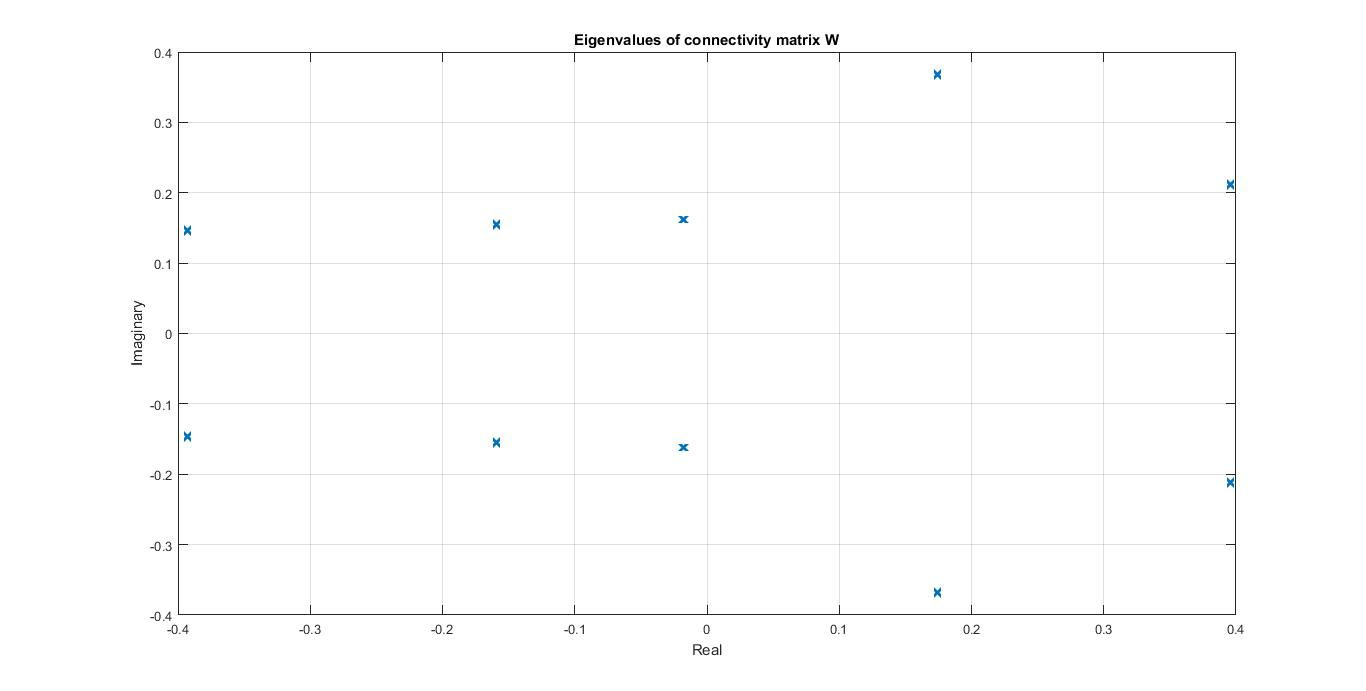
\includegraphics[width=0.9\textwidth]{Section1/Part2/Retry/Q2a_ii.jpg}
		\caption{Caption \label{Q2a_ii}}
	\end{center}
\end{figure}

iii. Equilibrium firing rates
\begin{figure}[H] 
	\begin{center}
		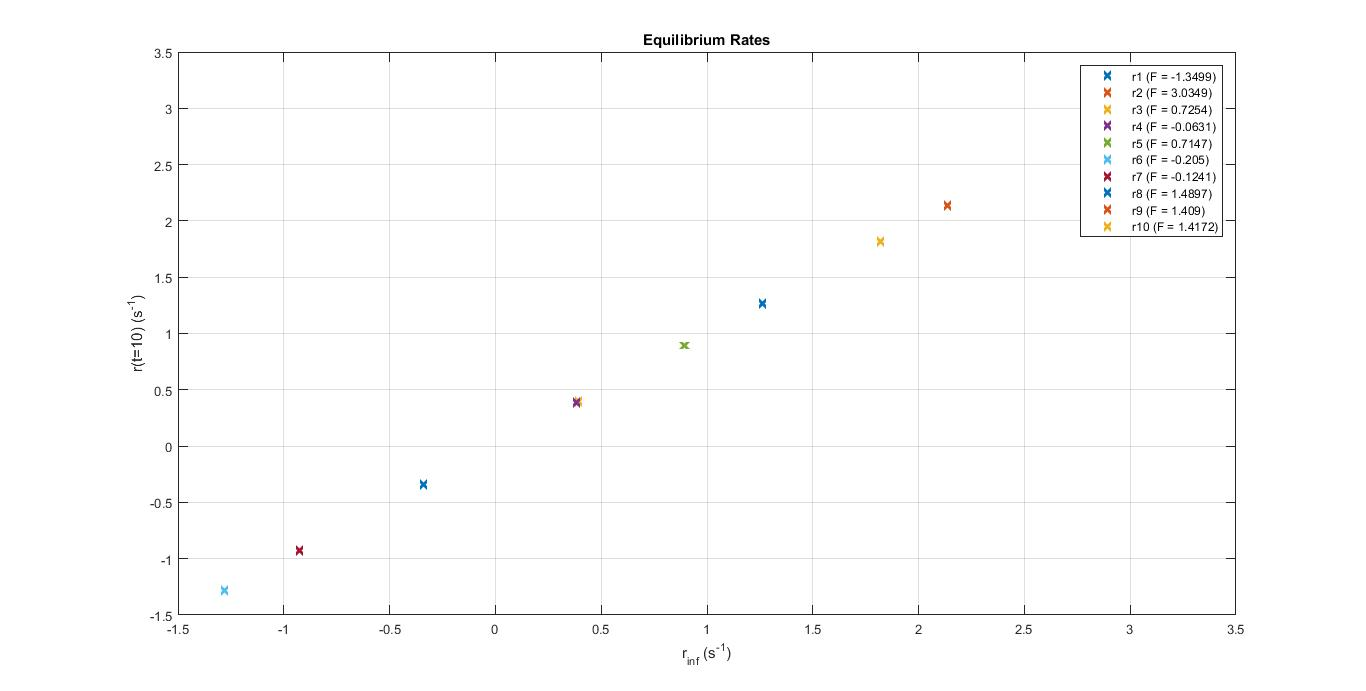
\includegraphics[width=0.9\textwidth]{Section1/Part2/Retry/Q2a_iii.jpg}
		\caption{Caption \label{Q2a_iii}}
	\end{center}
\end{figure}


\subsubsection{Firing rates with $g = 2$}
i. 
\begin{figure}[H] 
	\begin{center}
		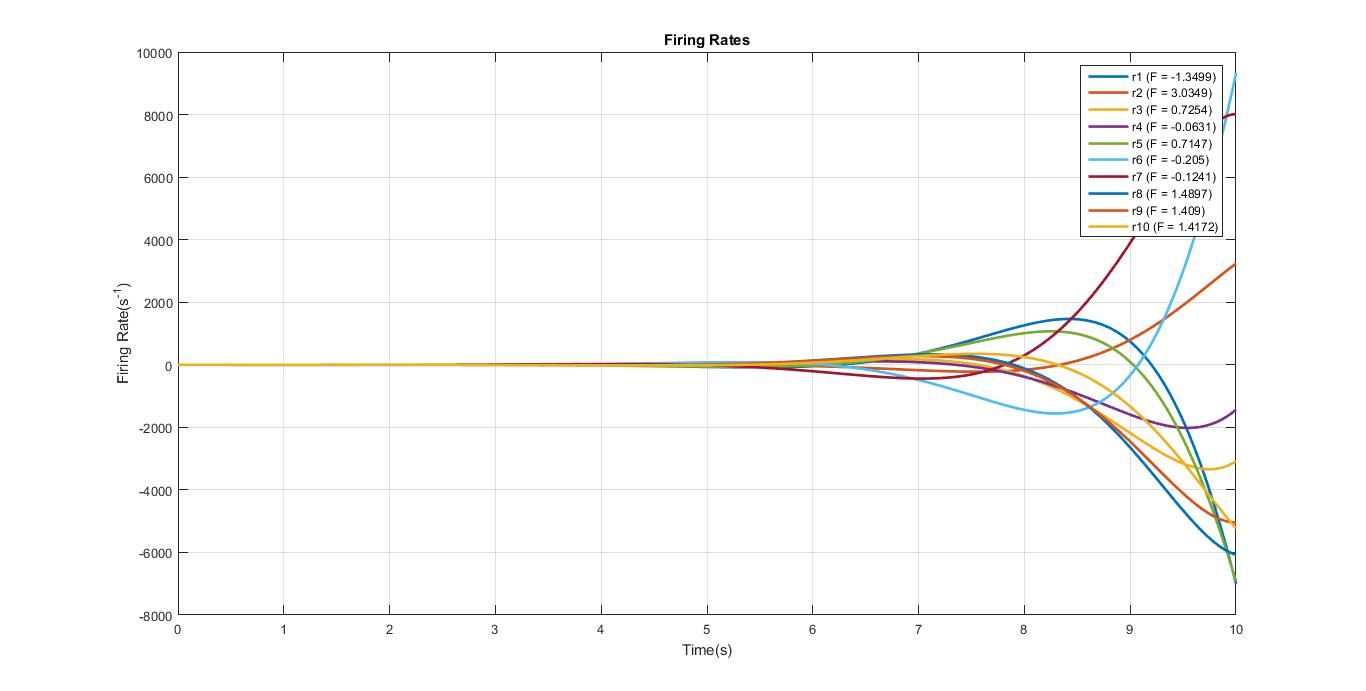
\includegraphics[width=0.9\textwidth]{Section1/Part2/Retry/Q2a_i_g2.jpg}
		\caption{Caption \label{Q2a_i_g2}}
	\end{center}
\end{figure}

ii. Eigenvalues of the recurrent connectivity matrix $W$
\begin{figure}[H] 
	\begin{center}
		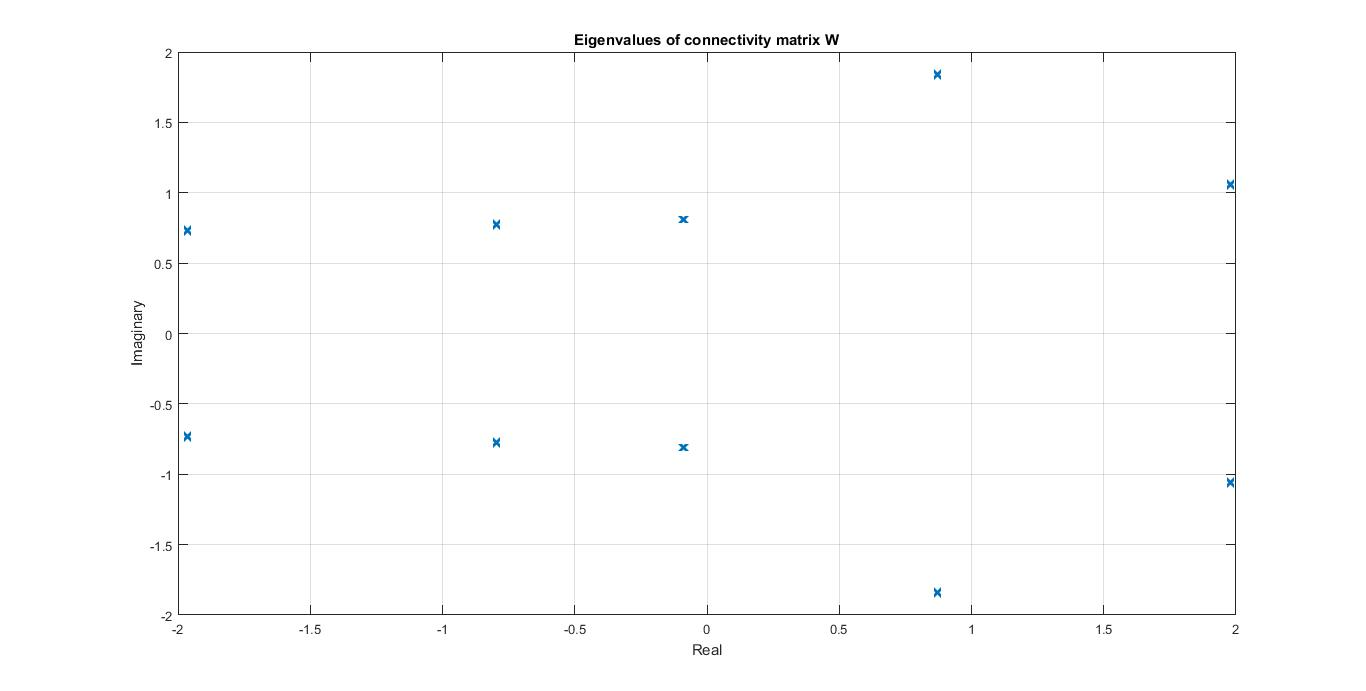
\includegraphics[width=0.9\textwidth]{Section1/Part2/Retry/Q2a_ii_g2.jpg}
		\caption{Caption \label{Q2a_ii_g2}}
	\end{center}
\end{figure}

iii. Equilibrium firing rates
\begin{figure}[H] 
	\begin{center}
		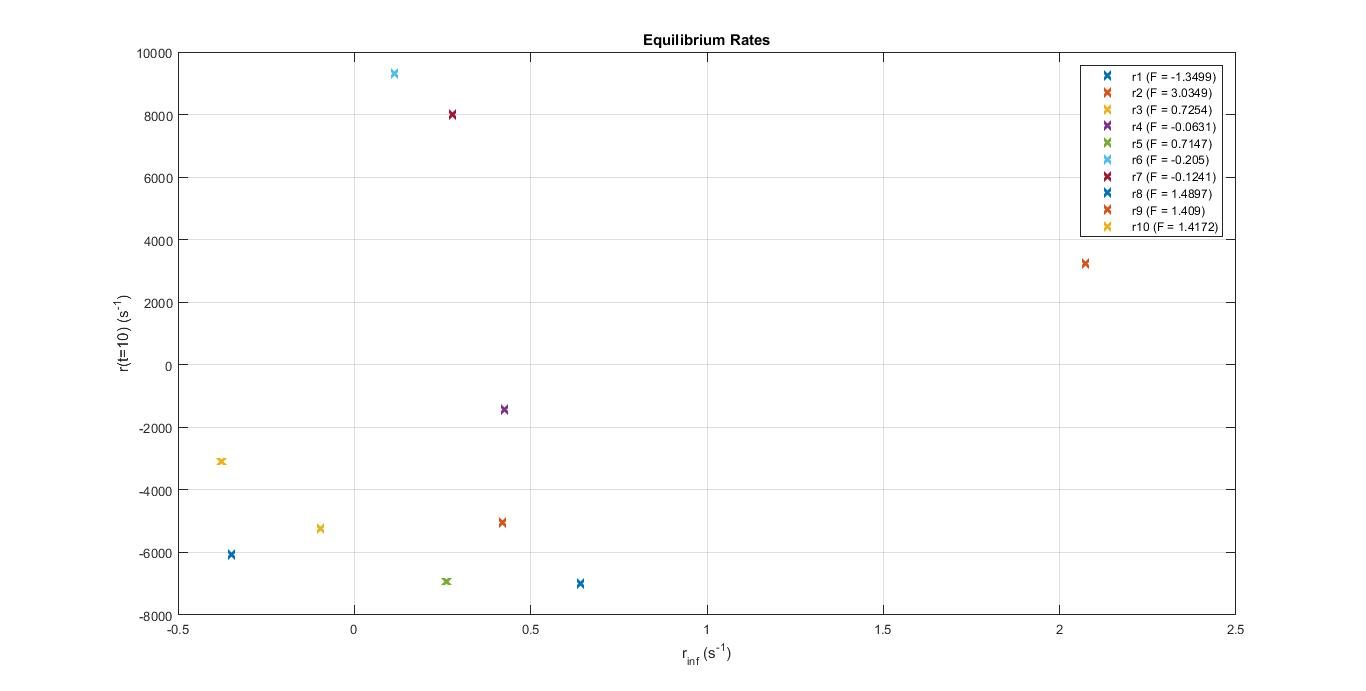
\includegraphics[width=0.9\textwidth]{Section1/Part2/Retry/Q2a_iii_g2.jpg}
		\caption{Caption \label{Q2a_iii_g2}}
	\end{center}
\end{figure}

\subsubsection{Firing rates with $g = 0.95$}
i. 
\begin{figure}[H] 
	\begin{center}
		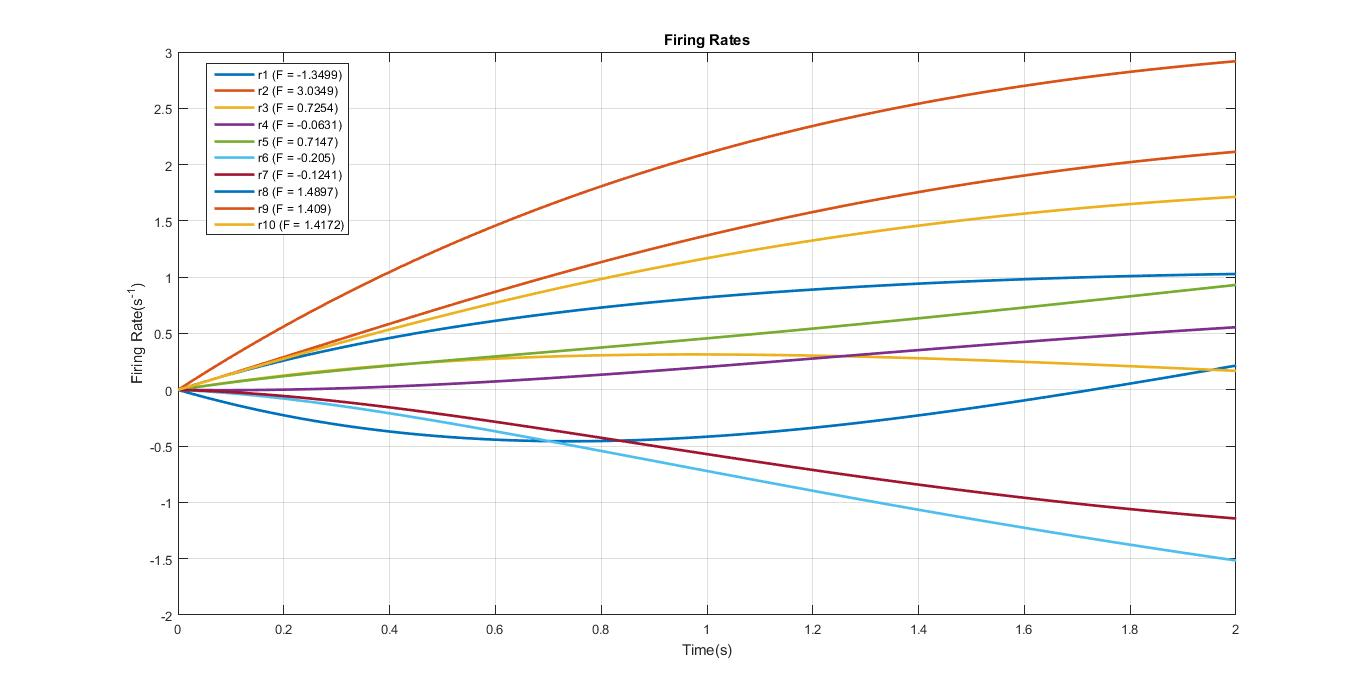
\includegraphics[width=0.9\textwidth]{Section1/Part2/Retry/Q2a_i_gInt.jpg}
		\caption{Caption \label{Q2a_i_g2}}
	\end{center}
\end{figure}

ii. Eigenvalues of the recurrent connectivity matrix $W$
\begin{figure}[H] 
	\begin{center}
		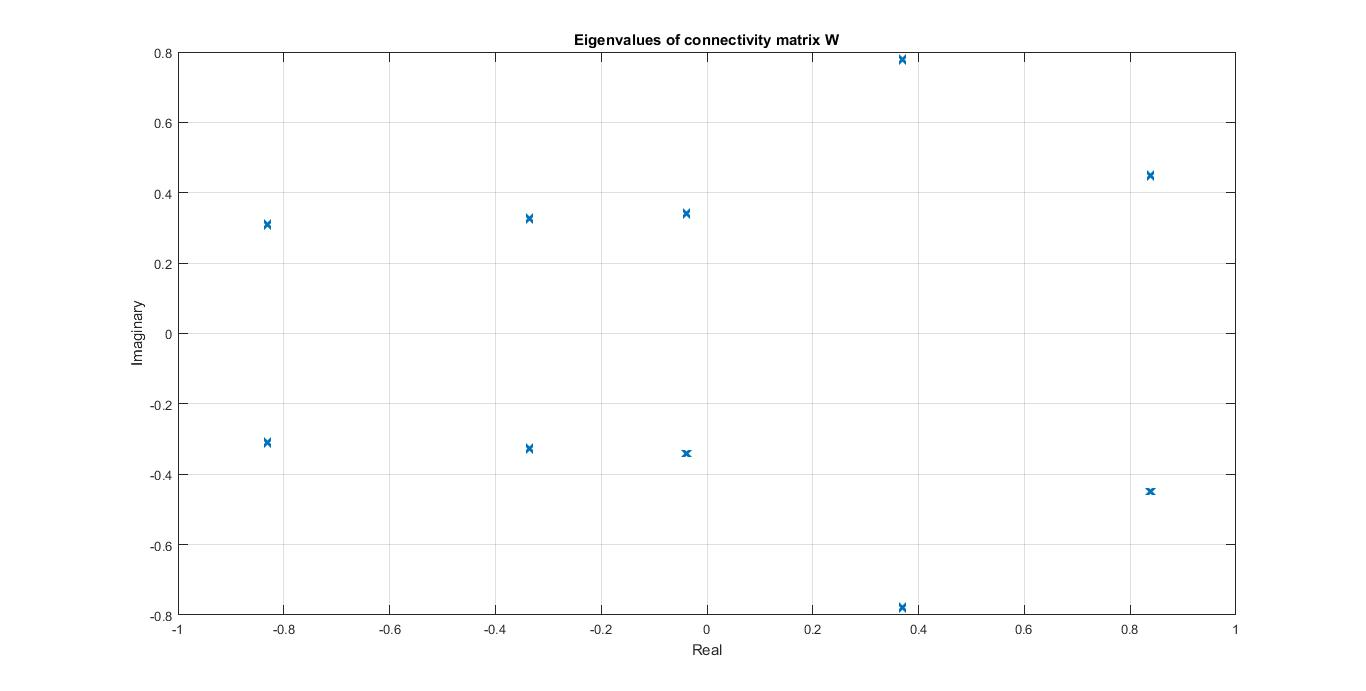
\includegraphics[width=0.9\textwidth]{Section1/Part2/Retry/Q2a_ii_gInt.jpg}
		\caption{Caption \label{Q2a_ii_g2}}
	\end{center}
\end{figure}

iii. Equilibrium firing rates
\begin{figure}[H] 
	\begin{center}
		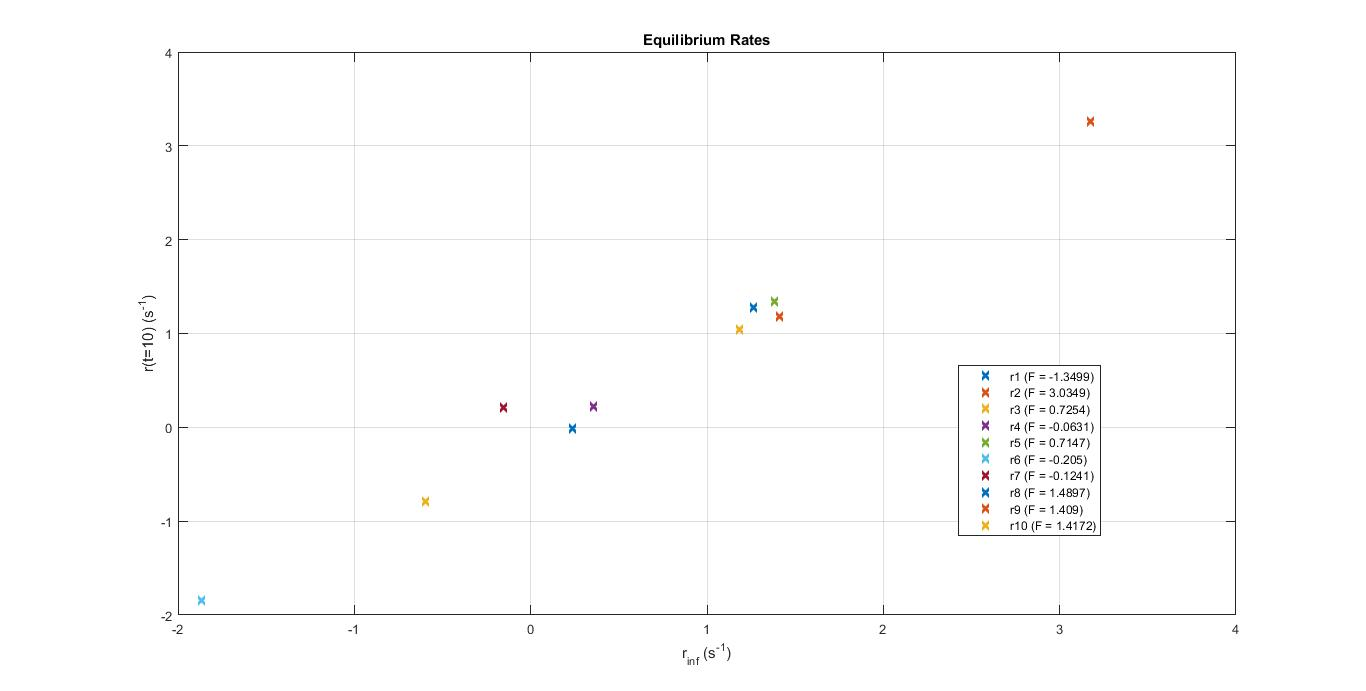
\includegraphics[width=0.9\textwidth]{Section1/Part2/Retry/Q2a_iii_gInt.jpg}
		\caption{Caption \label{Q2a_iii_g2}}
	\end{center}
\end{figure}
	
\subsection{Visual cortex model}

\subsubsection{Denoising}	
i. Noisy input
\begin{figure}[H] 
	\begin{center}
		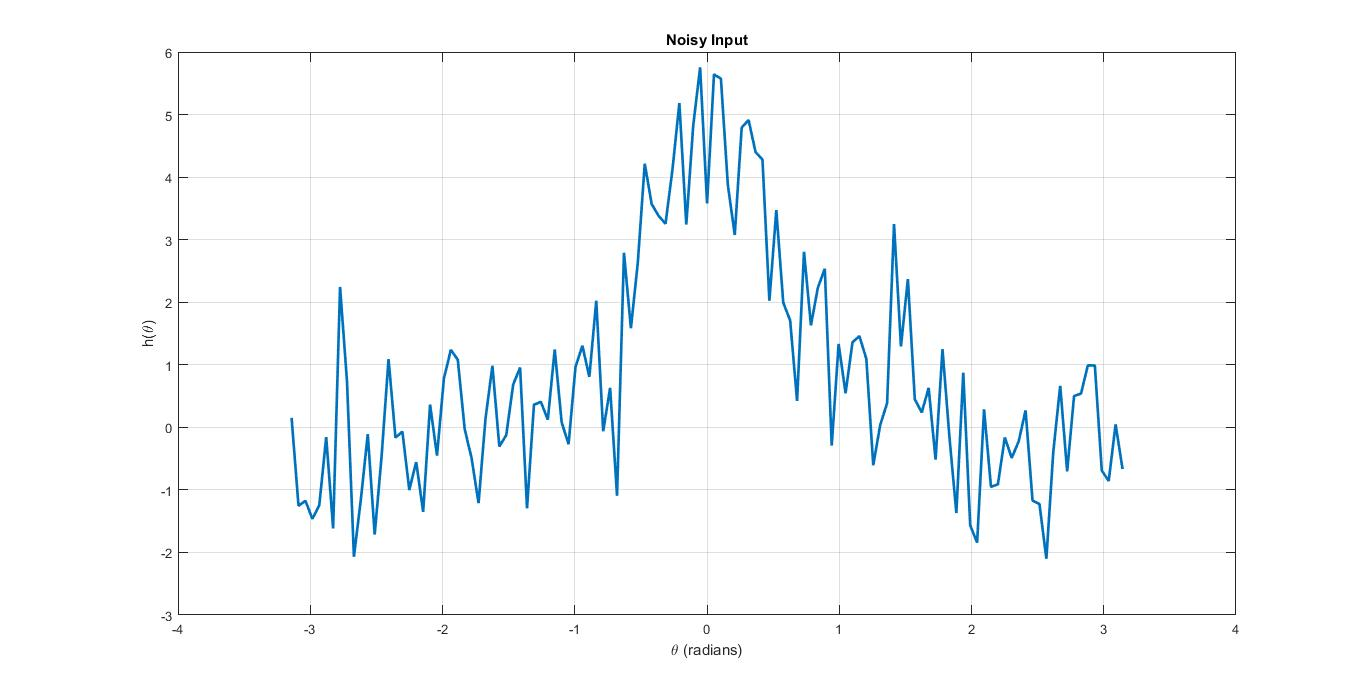
\includegraphics[width=0.9\textwidth]{Section1/Part3/3a_i.jpg}
		\caption{Caption \label{Q2a_iii_g2}}
	\end{center}
\end{figure}

ii. Equilibrium population firing rate
\begin{figure}[H] 
	\begin{center}
		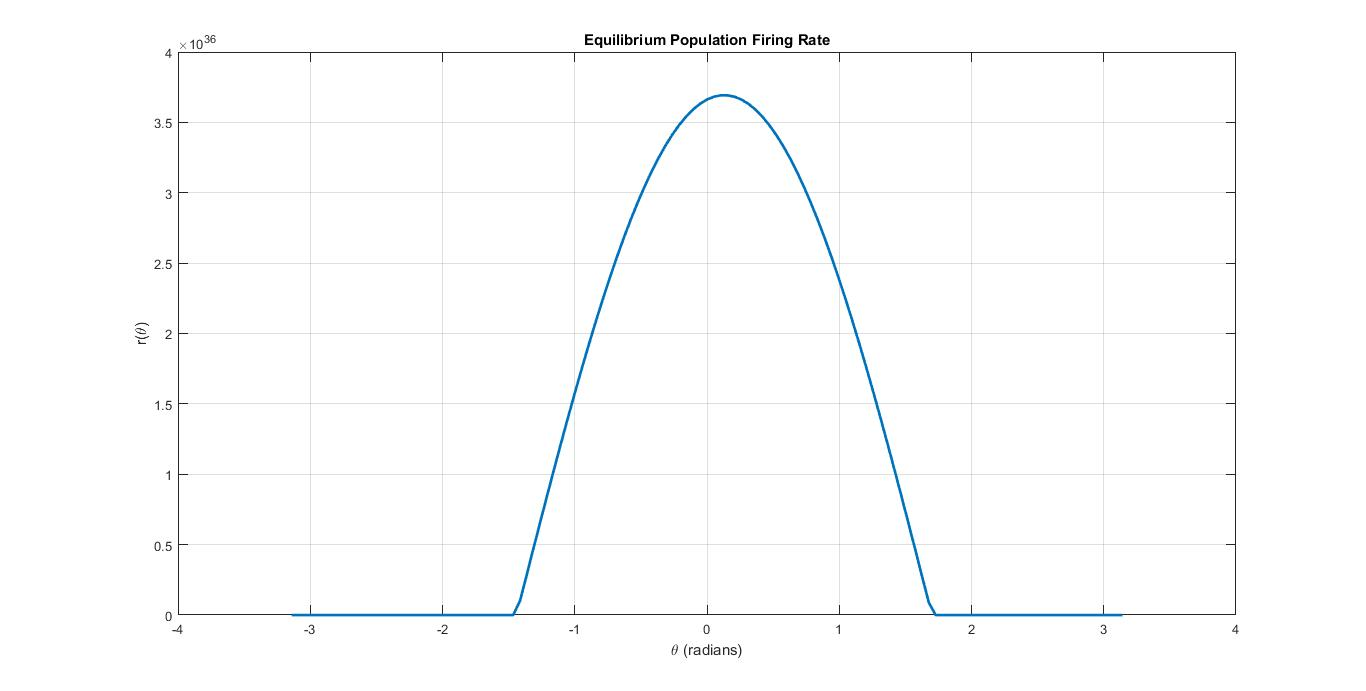
\includegraphics[width=0.9\textwidth]{Section1/Part3/3a_ii.jpg}
		\caption{Caption \label{Q2a_iii_g2}}
	\end{center}
\end{figure}

\subsubsection{Gain modulation}
i. Input
\begin{figure}[H] 
	\begin{center}
		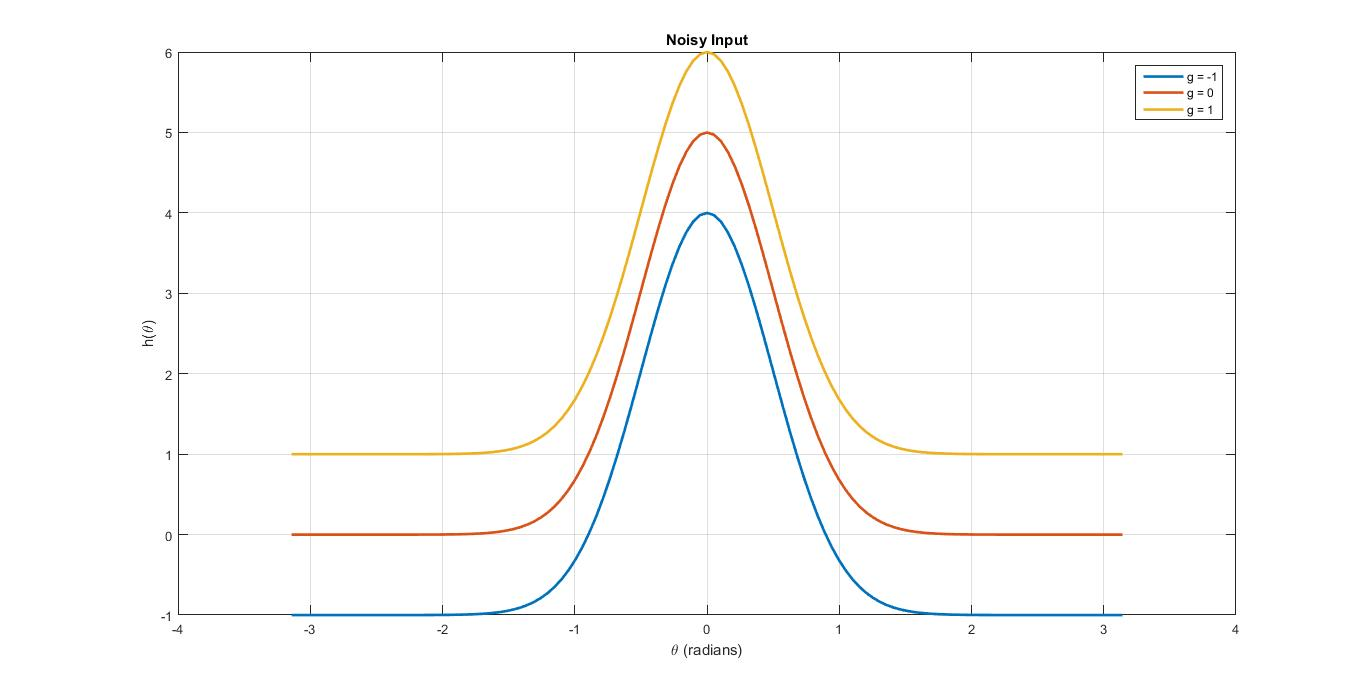
\includegraphics[width=0.9\textwidth]{Section1/Part3/3b_i.jpg}
		\caption{Caption \label{Q2a_iii_g2}}
	\end{center}
\end{figure}

ii. Equilibrium population firing rate
\begin{figure}[H] 
	\begin{center}
		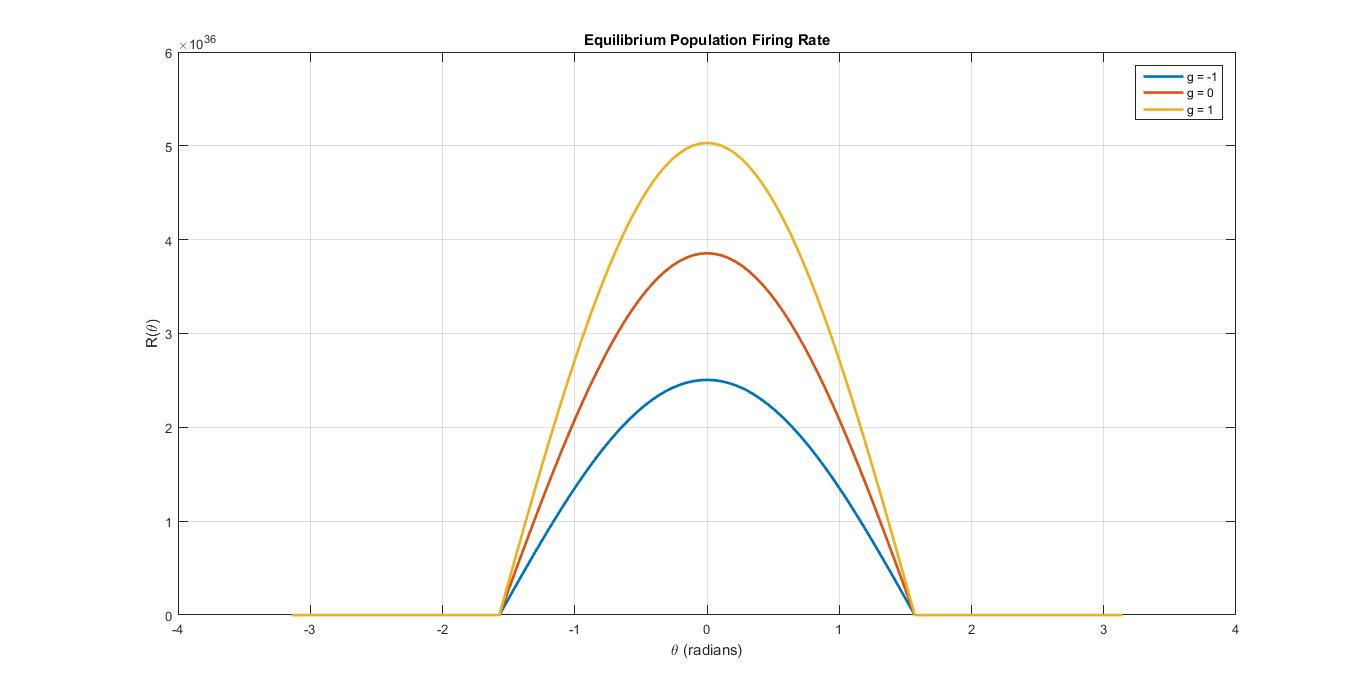
\includegraphics[width=0.9\textwidth]{Section1/Part3/3b_ii.jpg}
		\caption{Caption \label{Q2a_iii_g2}}
	\end{center}
\end{figure}

\subsubsection{Winner-takes-all input selection and sustained activity}
i. Input
\begin{figure}[H] 
	\begin{center}
		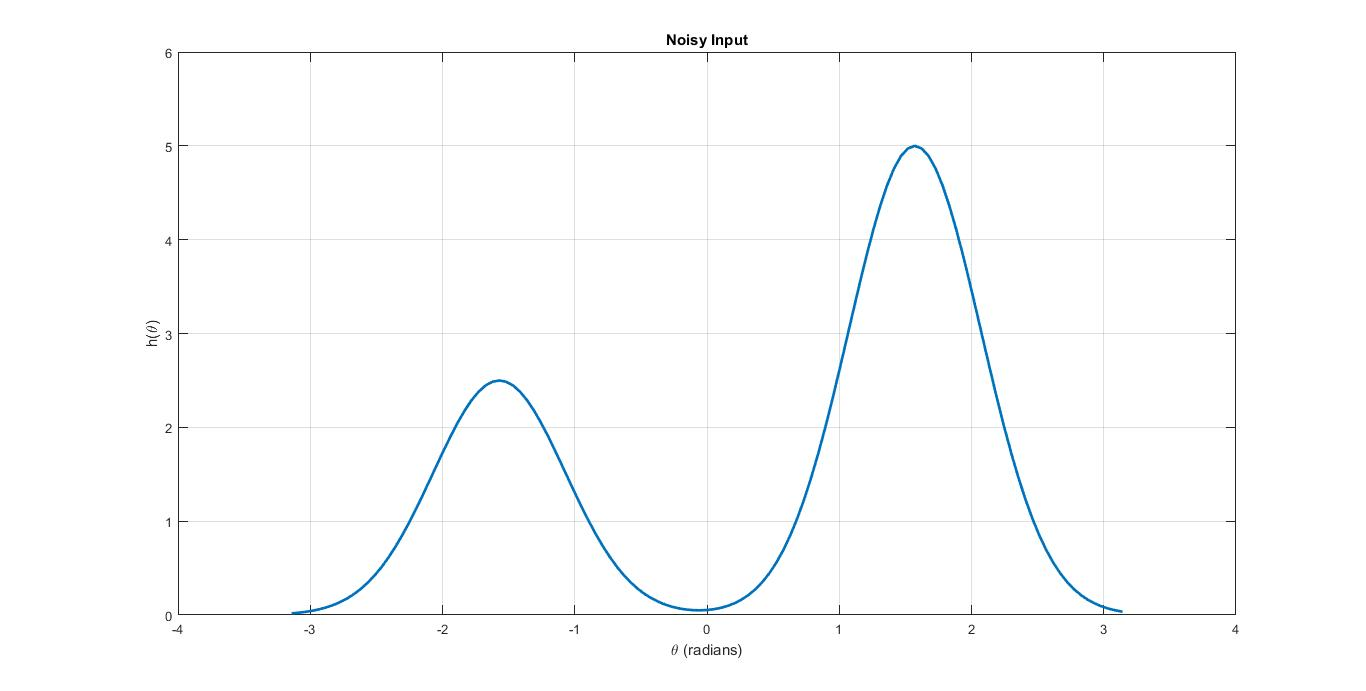
\includegraphics[width=0.9\textwidth]{Section1/Part3/3c_i.jpg}
		\caption{Caption \label{Q2a_iii_g2}}
	\end{center}
\end{figure}

ii. Equilibrium population firing rate
\begin{figure}[H] 
	\begin{center}
		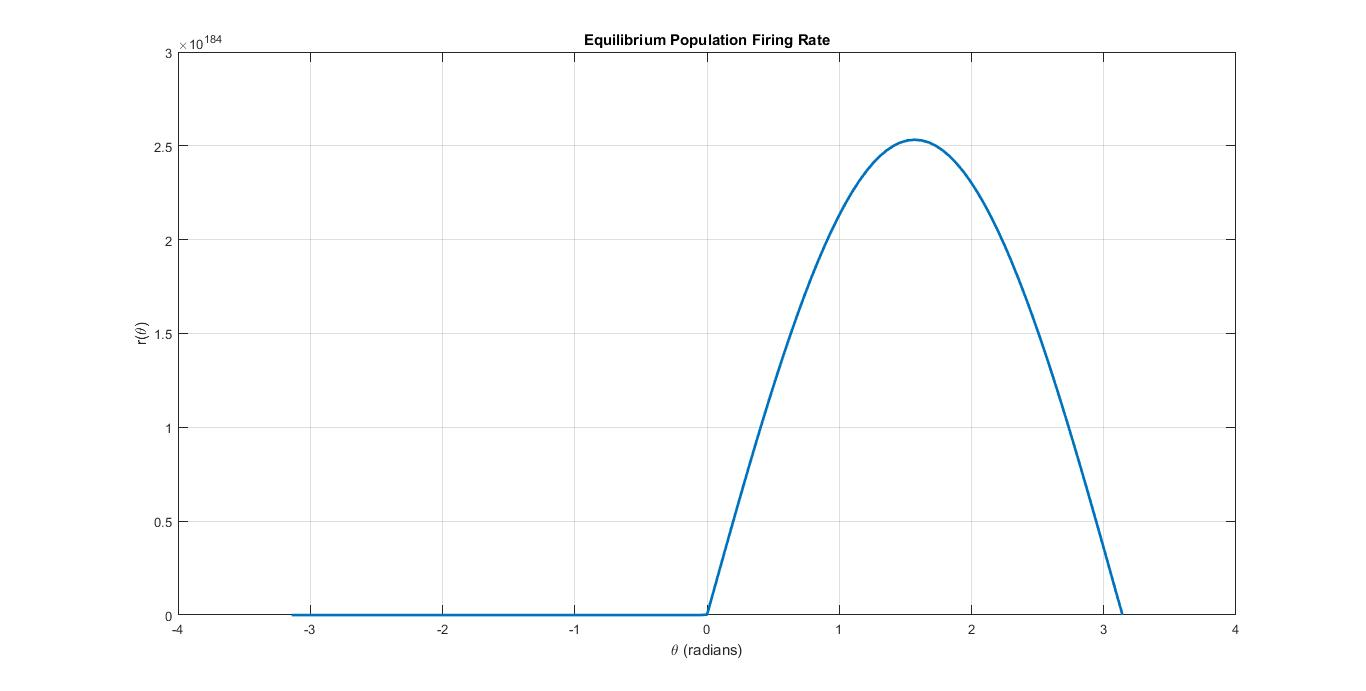
\includegraphics[width=0.9\textwidth]{Section1/Part3/3c_ii.jpg}
		\caption{Caption \label{Q2a_iii_g2}}
	\end{center}
\end{figure}

iii. Sustained activity
\begin{figure}[H] 
	\begin{center}
		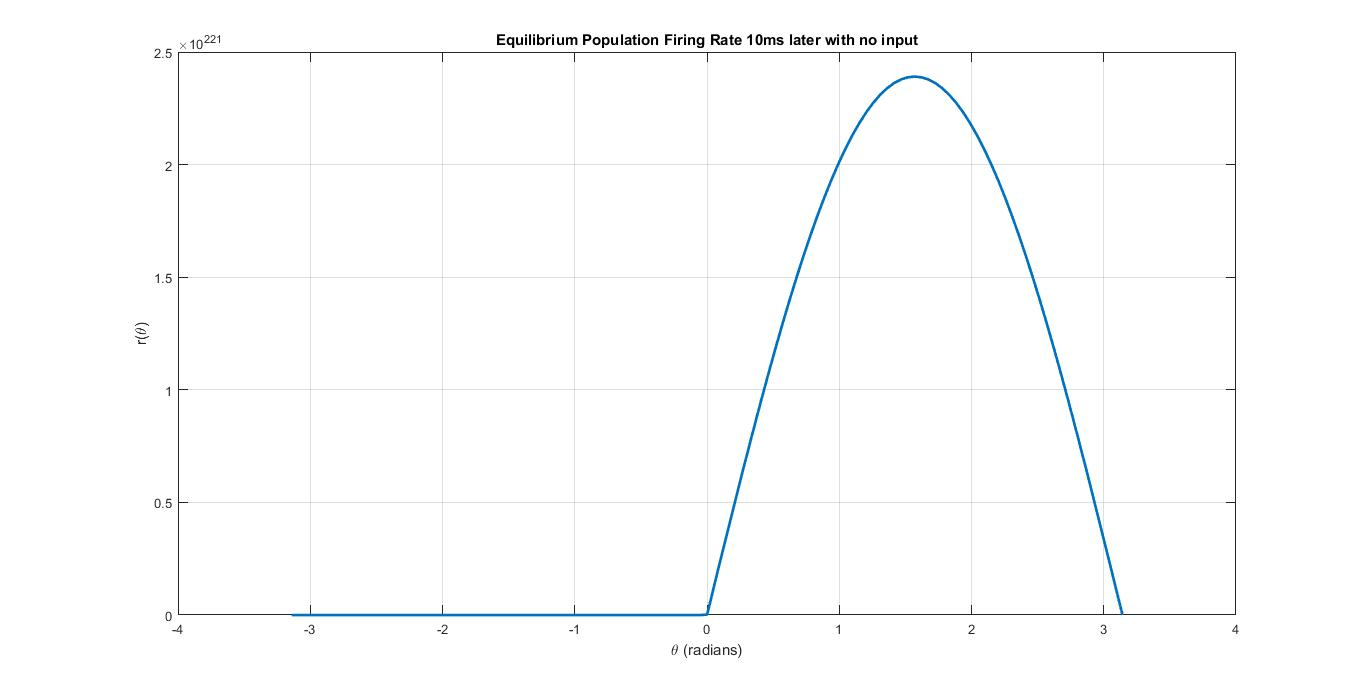
\includegraphics[width=0.9\textwidth]{Section1/Part3/3c_iii.jpg}
		\caption{Caption \label{Q2a_iii_g2}}
	\end{center}
\end{figure}

\section{The asynchronous \& irregular state of cortical circuits}
\subsubsection{Generating Poisson spike trains}
\begin{figure}[H] 
	\begin{center}
		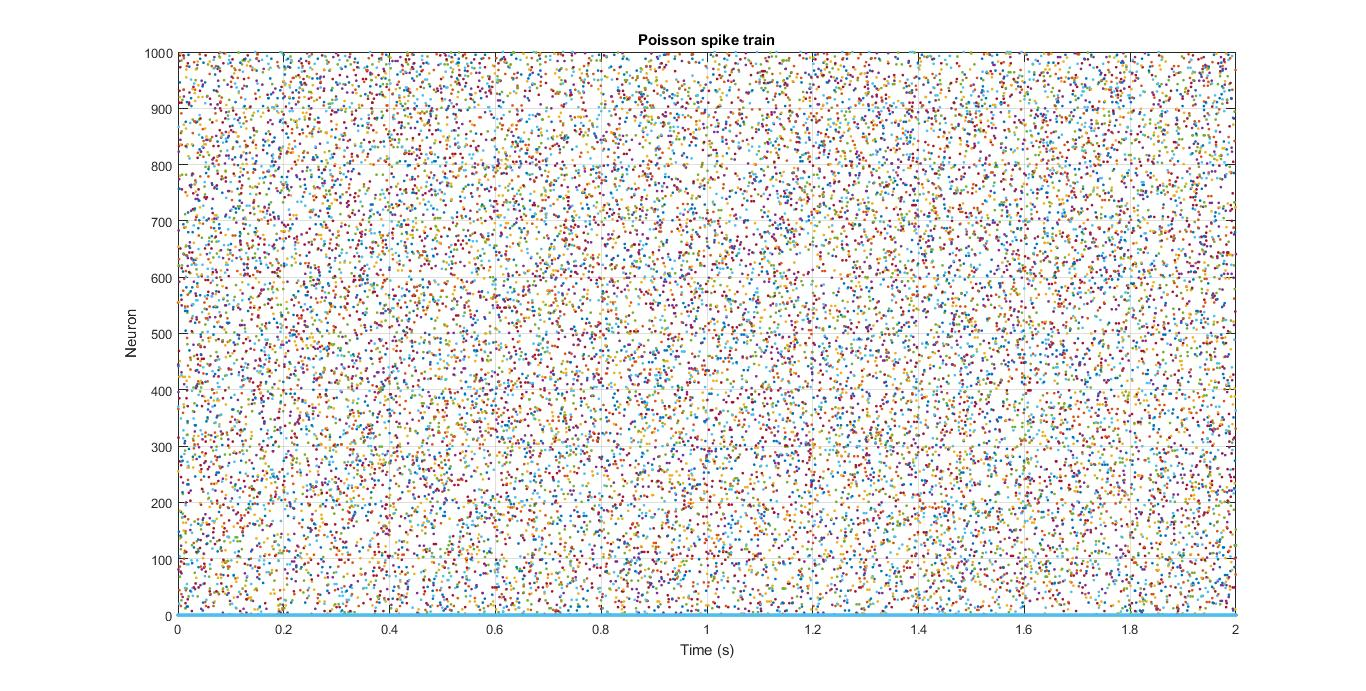
\includegraphics[width=0.9\textwidth]{Section2/1a.jpg}
		\caption{Caption \label{Q2a_iii_g2}}
	\end{center}
\end{figure}

\subsubsection{Single LIF neuron with one input spike train}

\begin{figure}[H] 
	\begin{center}
		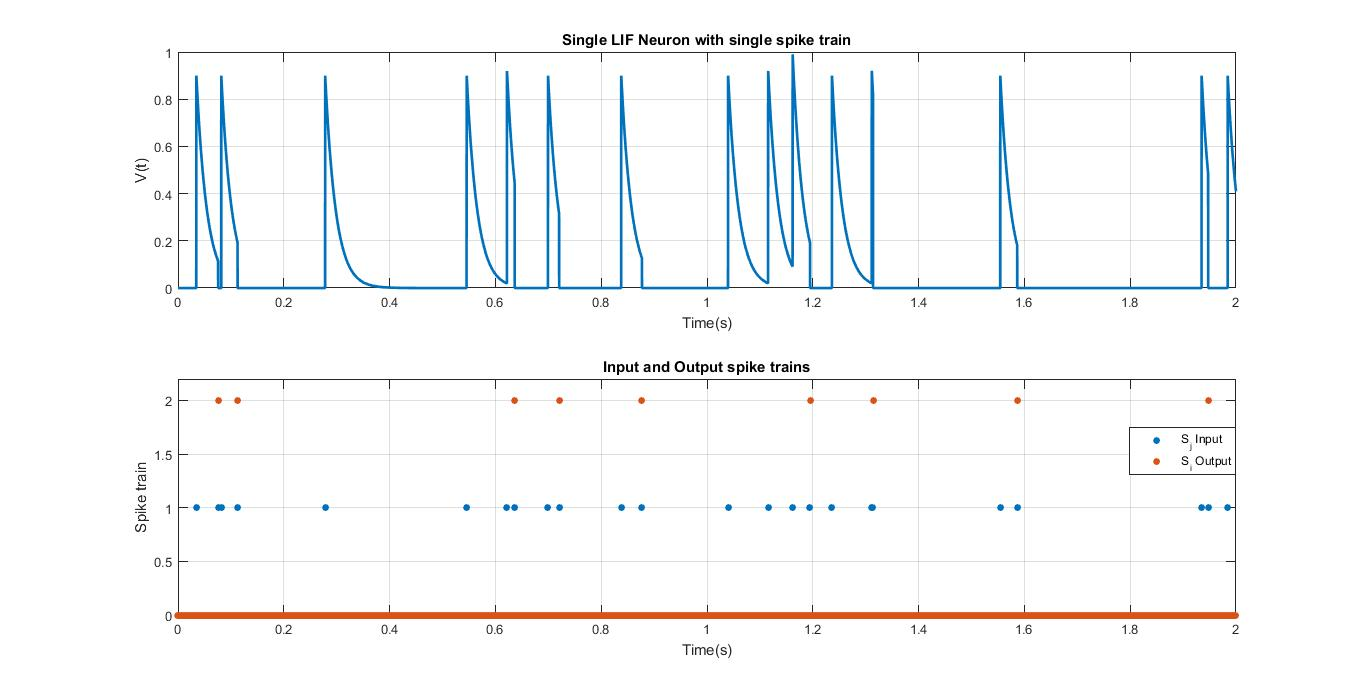
\includegraphics[width=0.9\textwidth]{Section2/2a.jpg}
		\caption{(a) Membrane potential dynamics \label{Q2a_iii_g2}}
	\end{center}
\end{figure}

\subsubsection{Single LIF neuron with many input spike train}
(a)
\begin{figure}[H] 
	\begin{center}
		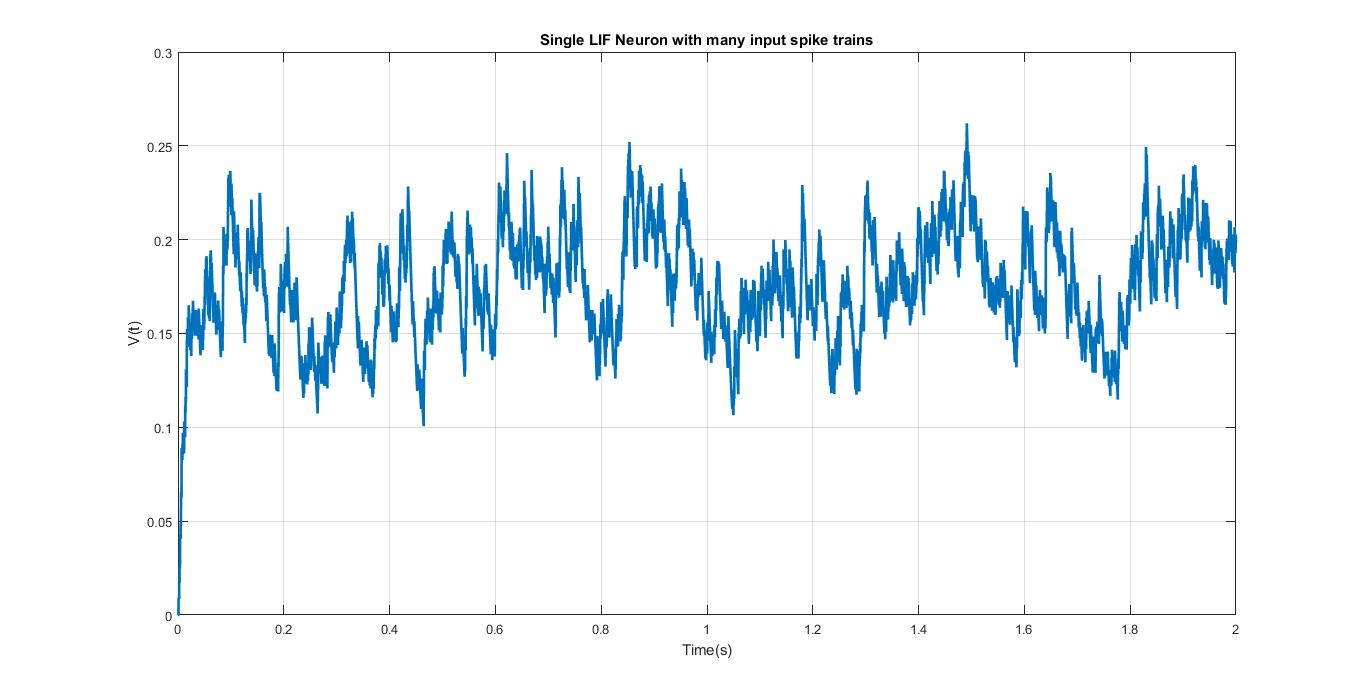
\includegraphics[width=0.9\textwidth]{Section2/3a_i.jpg}
		\caption{(a) Membrane potential dynamics without spike-reset ($w = 0.9$)\label{Q2a_iii_g2}}
	\end{center}
\end{figure}
	
\begin{figure}[H] 
		\begin{center}
			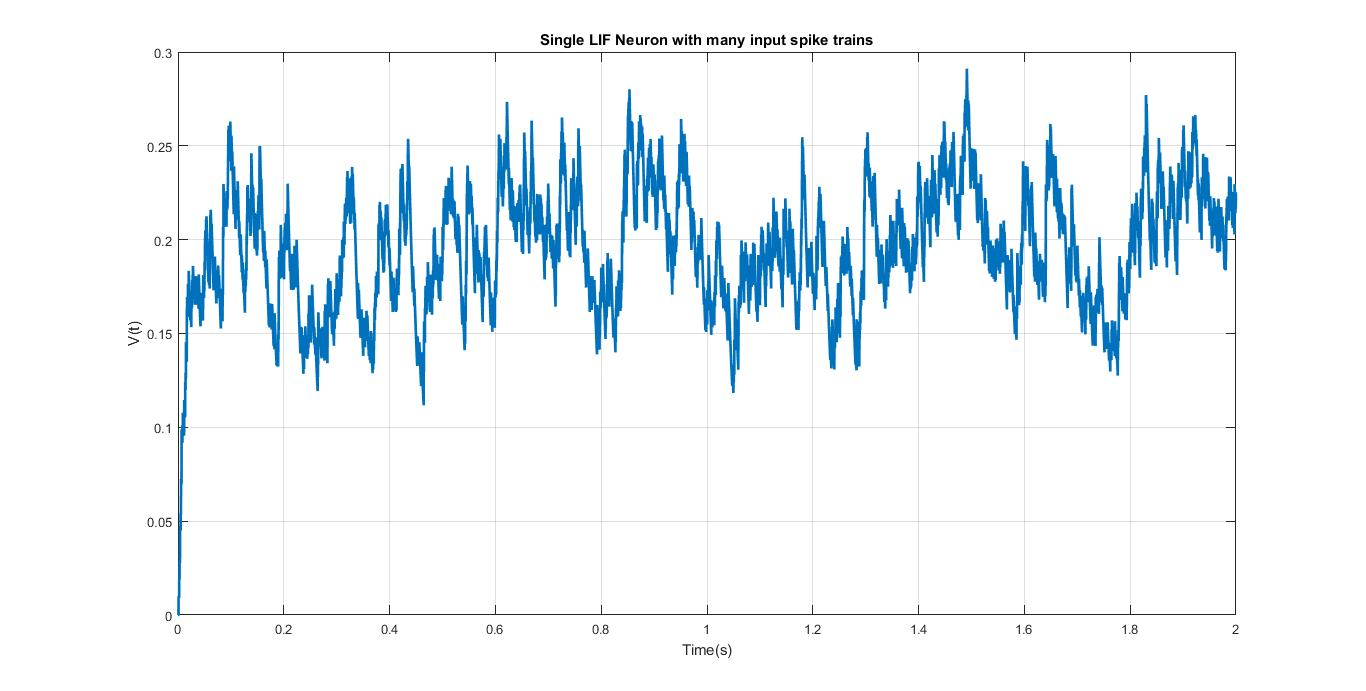
\includegraphics[width=0.9\textwidth]{Section2/3a_ii(w1).jpg}
			\caption{(a) Membrane potential dynamics without spike-reset ($w = 1$)\label{Q2a_iii_g2}}
		\end{center}
\end{figure}

(b) 
%\begin{displaymath}
%\begin{align*}
%h(t) = \frac{w}{K} \sum_{j = 1}^{K} S_{j}(t) \\
%\mathbb{E}[h(t)] = \mathbb{E}[\frac{w}{K} \sum_{j = 1}^{K} S_{j}(t)] \\
%				 = \frac{w}{K} \sum_{j = 1}^{K} \mathbb{E}[S_{j}(t)] \\
%				 = wr_{x}
%
%\end{align*}

\begin{align*}
\
h(t) = \frac{w}{K} \sum_{j = 1}^{K} S_{j}(t) \\
\mathbb{E}[h(t)] = \mathbb{E}[\frac{w}{K} \sum_{j = 1}^{K} S_{j}(t)] \\
= \frac{w}{K} \sum_{j = 1}^{K} \mathbb{E}[S_{j}(t)]\\
= \frac{w}{K} \sum_{j = 1}^{K} r_{X} \\
= wr_{X} 
\
\end{align*}

\begin{align*}

Var[h(t)] = \mathbb{E}[h(t)^2] - \mathbb{E}[h(t)]^2
\
\end{align*}




%\end{displaymath}

%\begin{gather}
%a + b = c \\ 
%a = c - b
%\end{gather}

\end{document}